\documentclass[11pt]{beamer}
\usetheme{Warsaw}
\usepackage[utf8]{inputenc}
\usepackage[english]{babel}
\usepackage{amsmath}
\usepackage{amsfonts}
\usepackage{amssymb}

%expectations
\newcommand{\expect}{\mathbb{E}}

\AtBeginSection[]{
  \begin{frame}
  \vfill
  \centering
  \begin{beamercolorbox}[sep=8pt,center,shadow=true,rounded=true]{title}
    \usebeamerfont{title}\insertsectionhead\par%
  \end{beamercolorbox}
  \vfill
  \end{frame}
}


\begin{document}
%%%%%%%%%%%%%%%%%%%%%%%%%%%%%%%%%%%%%%%%%%%%%%%%%%%%%%%%
\begin{frame}
  \frametitle{}
  \begin{center}
    \textbf{\large MATH 4281 Risk Theory--Ruin and Credibility}\\
    \vspace{1cm}
    {\large  Start Module 2: Ruin Theory} \\
    \vspace{1cm}
    {\large  Feb 2, 2021}
    \end{center}
    \vspace{1cm}
\end{frame}
%%%%%%%%%%%%%%%%%%%%%%%%%%%%%%%%%%%%%%%%%%%%%%%%%%%%%%%%
\begin{frame}
\tableofcontents
\end{frame}
%%%%%%%%%%%%%%%%%%%%%%%%%%%%%%%%%%%%%%%%%%%%%%%%%%%%%%%%
\section{Recap and Motivation}
\begin{frame}{The Story so Far}

\begin{itemize}

\item As it stands now- the models we have studied have assumed a \alert{short time frame}.

\vfill

\item We have tried to model aggregate claims over say a week/month/year. 

\vfill

\item Assumed no \alert{Time Value of Money} or rigorous model for  \alert{Premiums}. 

\end{itemize}

\end{frame}
%%%%%%%%%%%%%%%%%%%%%%%%%%%%%%%%%%%%%%%%%%%%%%%%%%%%%%%%
\begin{frame}{Some Questions} 

\begin{itemize}

\item[Q1] What happens if we can't pay all the claims?

\vfill

\item[Q2] How do we set premiums to guarantee that we can?

\vfill

\item[Q3] How does \alert{Time} factor in to this?

\end{itemize}
\vfill
\begin{center}
\textbf{These are the questions that we will explore in this module}
\end{center}

\end{frame}
%%%%%%%%%%%%%%%%%%%%%%%%%%%%%%%%%%%%%%%%%%%%%%%%%%%%%%%%
\section{Stochastic Processes}
\subsection{Intro}
\begin{frame}{What is a Stochastic Process}

\begin{itemize}

\item Stochastic - from the Greek for "to aim" or "to guess". Generally adjective denoting "randomness" e.g:
\begin{itemize}
\item stochastic process (mathematics)
\item stochastic resonance (biology)
\item newsworthy "stochastic terrorism" (social sciences)
\item etc...
\end{itemize}

\vfill 

\item Process - Latin for "progression" 

\vfill 

\item Stochastic Process - stands to reason this is some progression of random events

\end{itemize}


\end{frame}
%%%%%%%%%%%%%%%%%%%%%%%%%%%%%%%%%%%%%%%%%%%%%%%%%%%%%%%%
\begin{frame}{What is a Stochastic Process}

\begin{itemize}
\item A \alert{\textit{stochastic process}} is any collection of
random variables $X\left( t\right) $, $t\in T$. This stochastic process is denoted as
\begin{equation*}
\left\{ X\left( t\right) ,t\in T\right\} .
\end{equation*}%

\vfill

\item We are interested in modelling the aggregate losses over a given period of time, not necessarily \alert{at one point}!

\vfill

\item For example: the aggregate loss \underline{\emph{process}} denoted by $\{S(t), t\ge0\},$ where $S(t)$ is the aggregate loss \alert{at time $t$}.
\end{itemize}

\end{frame}
%%%%%%%%%%%%%%%%%%%%%%%%%%%%%%%%%%%%%%%%%%%%%%%%%%%%%%%%
\begin{frame}{Independent Increments} 

A stochastic process $\{X (t), t\ge 0\}$ has \alert{\textit{independent increments
}} if:

\begin{itemize}
\item For all $t_0<t_{1}<t_{2}<\cdot \cdot \cdot <t_{n}$ the following RVs\footnote{RV = Random Variable} are independent:

$$X\left( t_{1}\right)-X\left( t_{0}\right) ,X\left( t_{2}\right) -X\left( t_{1}\right) ,...,%
X\left( t_{n}\right) -X\left( t_{n-1}\right) $$ 

\vfill

\item That is, future increases are independent of the past.


\end{itemize}

\end{frame}
%%%%%%%%%%%%%%%%%%%%%%%%%%%%%%%%%%%%%%%%%%%%%%%%%%%%%%%%
\begin{frame}{Stationary Increments} 

A stochastic process $\{X (t), t\ge 0\}$ has \alert{\textit{stationary increments }}
if:

\begin{itemize}

\item for all choices of $t_{1}$, $t_{2}$ and $\tau >0$:

$$ X\left( t_{2}+\tau \right) -X\left( t_{1}+\tau \right) \stackrel{d}{=} X\left( t_{2}\right) -X\left( t_{1}\right)$$

\vfill

\item Equivalently for $s<t$

$$ X\left( t \right) -X\left(s \right) \stackrel{d}{=} X\left( t-s \right)$$

\end{itemize}

\end{frame}
%%%%%%%%%%%%%%%%%%%%%%%%%%%%%%%%%%%%%%%%%%%%%%%%%%%%%%%%
\begin{frame}{Counting process}

\begin{itemize}

\item A stochastic process $\left\{ N\left( t\right) ,t\geq 0\right\} $
is a \alert{\textit{counting process}} if it represents the number of events that
occur up to time $t.$

\vfill

\item Q: What is the significance of counting processes?

\vfill

\item A: We will use them to model the number of claims recived during a particular time. 

\end{itemize}

\end{frame}
%%%%%%%%%%%%%%%%%%%%%%%%%%%%%%%%%%%%%%%%%%%%%%%%%%%%%%%%
\begin{frame}{Counting process}

\noindent A counting process $\left\{ N\left( t\right) ,t\geq 0\right\} $
must satisfy:

\begin{enumerate}
\item $N\left( t\right) \geq 0$.

\vfill

\item $N\left( t\right) $ is integer-valued.

\vfill

\item $N\left( s\right) \leq N\left( t\right) $ for any $s<t$, i.e. it must
be non-decreasing.

\vfill

\item For $s<t$, $N\left( t\right) -N\left( s\right) $ is the number of
events that have occurred in the interval $(s,t].$\newpage
\end{enumerate}

\end{frame}
%%%%%%%%%%%%%%%%%%%%%%%%%%%%%%%%%%%%%%%%%%%%%%%%%%%%%%%%
\subsection{Poisson Process}
\begin{frame}A counting process $\left\{ N\left( t\right) ,t\geq 0\right\} $ is
a \alert{\textit{Poisson process}} with rate $\lambda $, for $\lambda >0$, if:

\begin{enumerate}
\item $N\left( 0\right) =0$;

\item it has independent increments; and

\item the number of events in any interval of length $t$ has a Poisson
distribution with mean $\lambda t$. That is, for all $s,t\geq 0$,$n=0,1,...$%
\begin{equation*}
\text{$\Pr $}\left[ N\left( t+s\right) -N\left( s\right) =n\right]
=e^{-\lambda t}\frac{\left( \lambda t\right) ^{n}}{n!}.
\end{equation*}%
\newpage
\end{enumerate}

\end{frame}
%%%%%%%%%%%%%%%%%%%%%%%%%%%%%%%%%%%%%%%%%%%%%%%%%%%%%%%%
\begin{frame}{A path (realization) of the Poisson  process}

\begin{columns}
\column{0.67\textwidth}
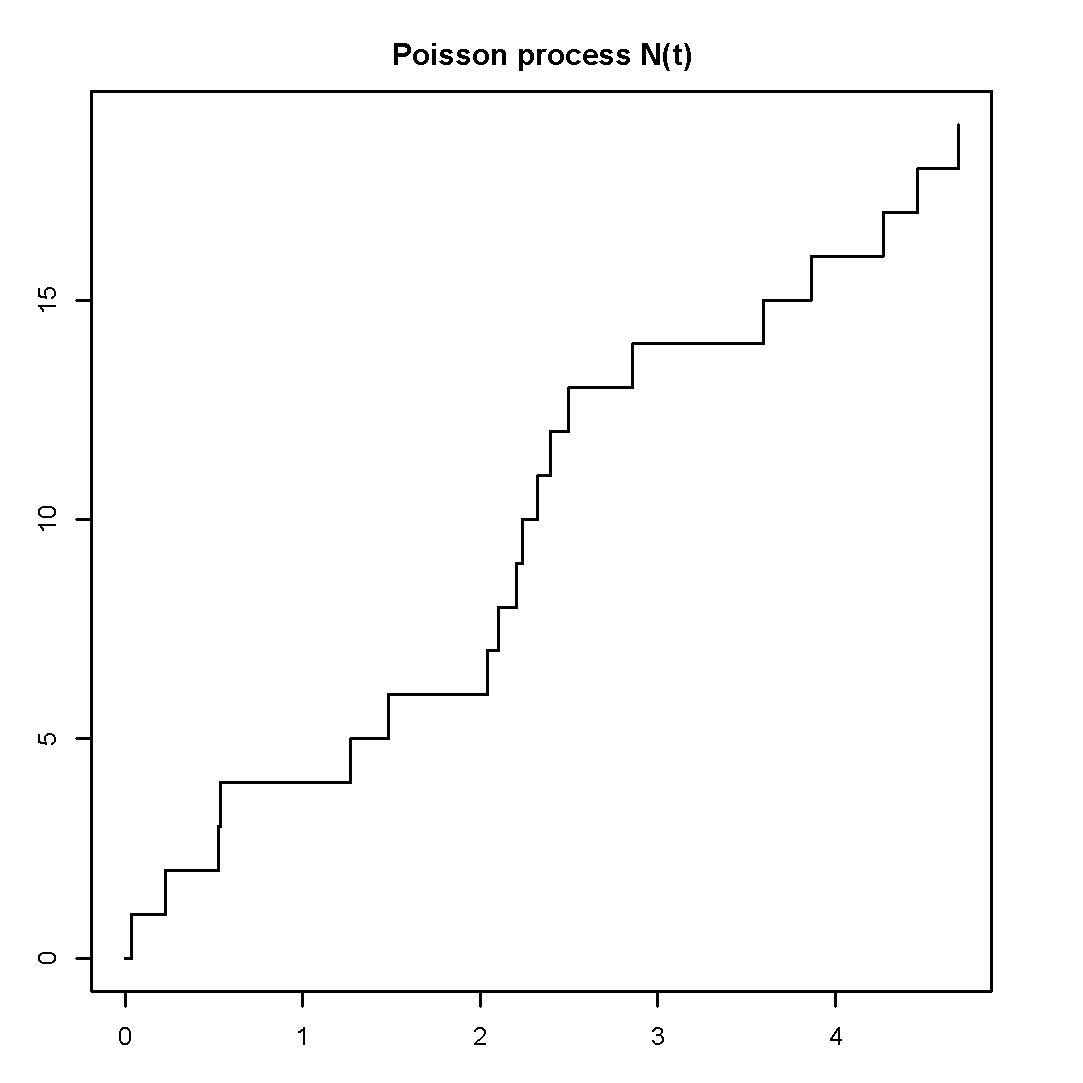
\includegraphics[scale=0.4]{Poisson}
\column{0.35\textwidth}
\begin{itemize}
\item Counting process
\item Step function
\item What is the \alert{arrival time}?
\end{itemize}
\end{columns}

\end{frame}
%%%%%%%%%%%%%%%%%%%%%%%%%%%%%%%%%%%%%%%%%%%%%%%%%%%%%%%%
\begin{frame}{A Noteworthy Characterization} 
\vspace{-3 cm}
Theorem: 
\begin{itemize}

\item Consider the time from the $i-1$th and $i$th jump $W_i$. 

\item That is $t=W_1 + ... + W_{N(t)}$

\item Then~$N(t+h)-N(t)\sim$~Poi$(\lambda h)$~iff~$W_i \sim\text{Exp}(1/\lambda)$

\end{itemize}
Proof:


\end{frame}
%%%%%%%%%%%%%%%%%%%%%%%%%%%%%%%%%%%%%%%%%%%%%%%%%%%%%%%%
\begin{frame}

\end{frame}
%%%%%%%%%%%%%%%%%%%%%%%%%%%%%%%%%%%%%%%%%%%%%%%%%%%%%%%%
\begin{frame}{A Noteworthy Characterization}
\vspace{-3 cm}
\begin{itemize}
\item Recall also that there is something special about the  distribution!
\item Exponential waiting times are \alert{Memoryless}
\end{itemize}
E.g: 




\end{frame}
%%%%%%%%%%%%%%%%%%%%%%%%%%%%%%%%%%%%%%%%%%%%%%%%%%%%%%%%
\begin{frame}{Zooming in on the process}
\vspace{- 2 cm}
Explain why the following are true:
\begin{eqnarray*}
P\left[ N\left( t+dt\right) -N\left( t\right) =1\left\vert N\left(s\right),0\leq s\leq t\right. \right]  &=&\lambda dt+o(dt) \\
P\left[ N\left( t+dt\right) -N\left( t\right) =0\left\vert N\left(s\right),0\leq s\leq t\right. \right]  &=&1-\lambda dt +o(dt)\\
P\left[ N\left( t+dt\right) -N\left( t\right) \geq 2\left\vert N\left( s\right) ,0\leq s\leq t\right. \right]  &=&o(dt)
\end{eqnarray*}
\vfill
\end{frame}
%%%%%%%%%%%%%%%%%%%%%%%%%%%%%%%%%%%%%%%%%%%%%%%%%%%%%%%%
\begin{frame}

\end{frame}
%%%%%%%%%%%%%%%%%%%%%%%%%%%%%%%%%%%%%%%%%%%%%%%%%%%%%%%%
\begin{frame}{Properties of the Poisson process: Summary}

If $\left\{ N\left( t\right) ,t\geq 0\right\} $ is a \textit{%
Poisson process} with rate $\lambda $, for $\lambda >0$, then
\begin{enumerate}
\item $N\left( 0\right) =0$;

\item it has independent \alert{and} stationary increments;

\item It can never have  more than 1 jump at a time! That is:
\begin{equation*}
\Pr \left[ N\left( t+h\right) -N\left( t\right) =0\right] =e^{-\lambda h}=1-\lambda h+o\left(
h\right)
\end{equation*}%
\begin{equation*}
\Pr \left[ N\left( t+h\right) -N\left( t\right) =1\right] =\lambda he^{-\lambda h}=\lambda h+o\left(
h\right)
\end{equation*}%

and 

\begin{equation*}
\Pr \left[ N\left( t+h\right) -N\left( t\right) \geq 2\right] =o\left(
h\right)
\end{equation*}


\item The time between two consecutive jumps follows the Exponential($\lambda$) distribution.
\end{enumerate}

\end{frame}
%%%%%%%%%%%%%%%%%%%%%%%%%%%%%%%%%%%%%%%%%%%%%%%%%%%%%%%%
\begin{frame}{Brownian motion as the limit of a shifted Poisson process}
\begin{columns}
\column{0.55\textwidth}
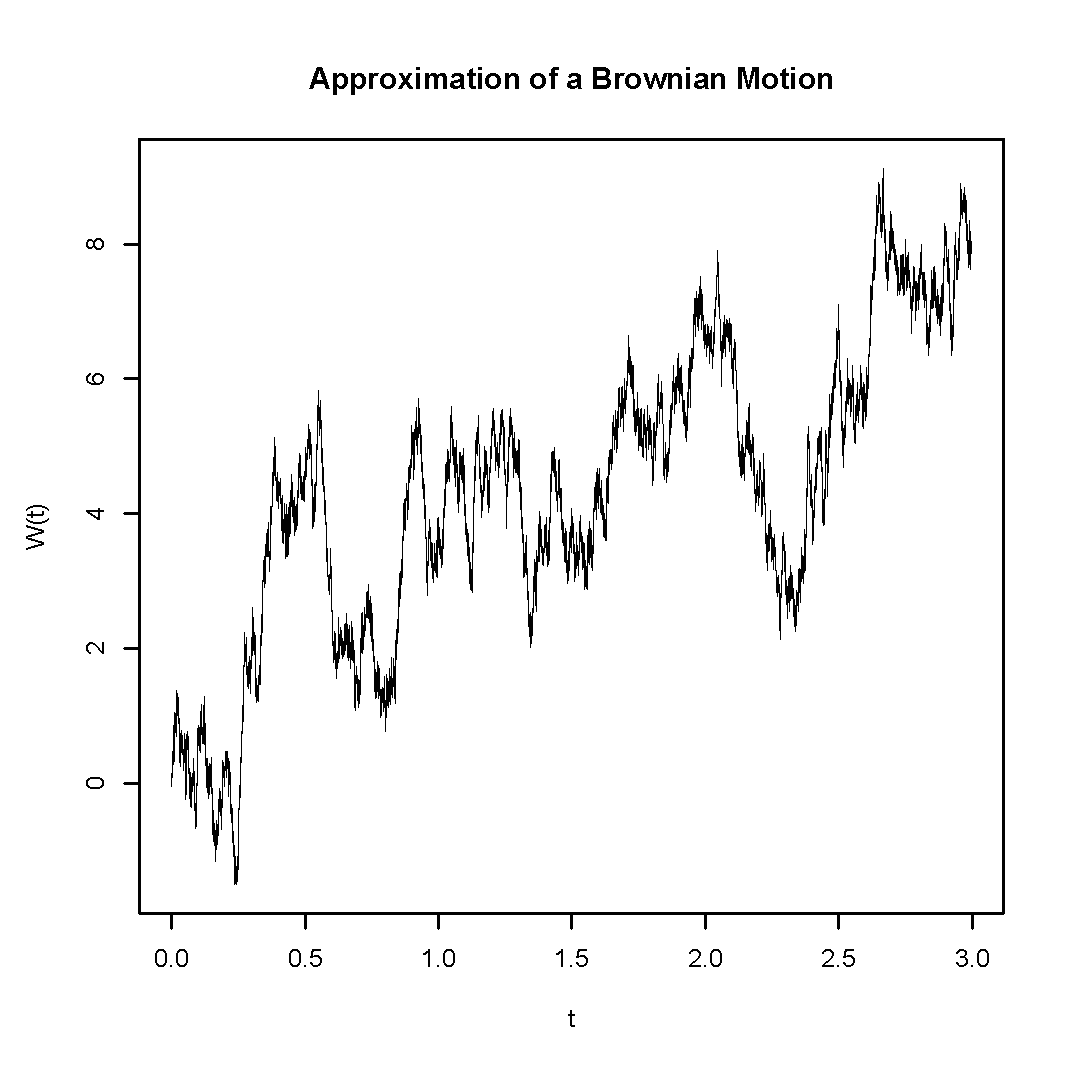
\includegraphics[width=\textwidth,bb=0 0 492 492]{exampleB2}
\vspace{-0.3cm}
{\small $$(\mu=2,\;\;\;\sigma=5,\text{ and }\tau=0.02)$$}
\column{0.55\textwidth}
Consider the following shifted Poisson process:
$$W(t)=\tau N(t) -ct.$$
Increments have moments
$$E[W(t+h)-W(t)]=(\tau \lambda -c)h \equiv \mu h,$$
$$Var(W(t+h)-W(t))=(\tau^2 \lambda)h \equiv \sigma^2 h.
$$
When $\tau \rightarrow 0$ for fixed $\mu$ and $\sigma^2$, $\{W(t)\}$ becomes a Brownian motion with parameters $\mu$ and $\sigma^2$.
\vspace{.2cm}
\end{columns}
\end{frame}
%%%%%%%%%%%%%%%%%%%%%%%%%%%%%%%%%%%%%%%%%%%%%%%%%%%%%%%%
\subsection{The compound Poisson process}
\begin{frame}

We define a \alert{Compound Poisson process} $\lbrace S(t), t\geq0 \rbrace$ like so:
$$S(t)=\sum_{i=1}^{N(t)}X_i.$$

Where:

\begin{itemize}

\item $\{N(t)\}$ is a Poisson process with parameter $\lambda$

\item $\{X_i\}$ are iid $\sim P(x)$


\end{itemize}

\end{frame}
%%%%%%%%%%%%%%%%%%%%%%%%%%%%%%%%%%%%%%%%%%%%%%%%%%%%%%%%
\begin{frame}{A path (realization) of the compound Poisson process}
\begin{columns}
\column{0.67\textwidth}

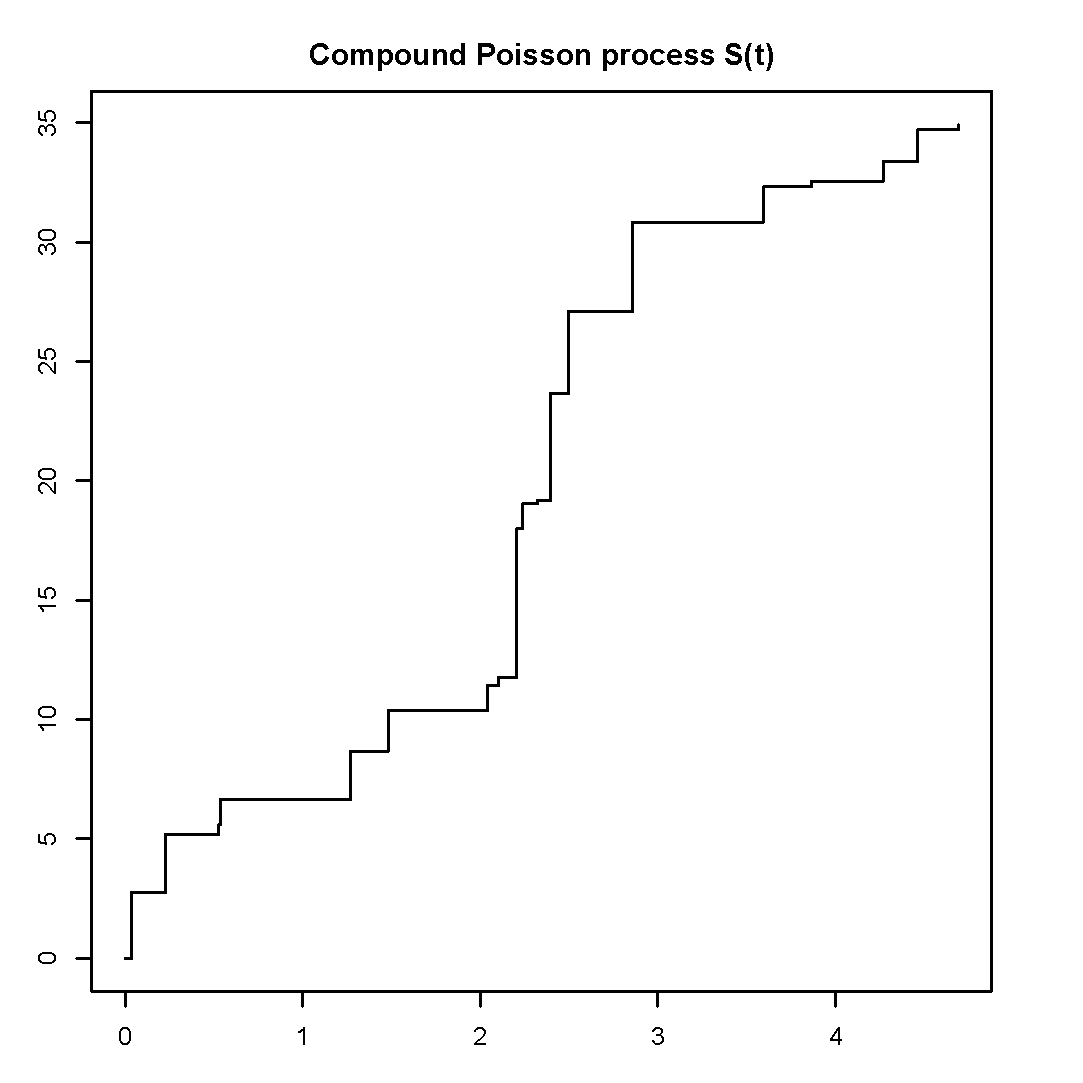
\includegraphics[width=\textwidth,bb=0 0 495 503]{cPoisson}

\column{0.35\textwidth}

\begin{itemize}
\item Now step $i$ has height $X_i$ instead of 1.

\item Increments $S(t+h)-S(t)\sim$
Compound Poisson$(\lambda h,P(x))$
\end{itemize}

\end{columns}
\end{frame}
%%%%%%%%%%%%%%%%%%%%%%%%%%%%%%%%%%%%%%%%%%%%%%%%%%%%%%%%
\begin{frame}
\vspace{-2 cm}
Mean and Variance of the compound Poisson process:
\begin{eqnarray*}
E [S (t)] = \lambda t E [ X ] , \quad \mbox{Var} [S (t)] = \lambda t E [ X^2 ] .
\end{eqnarray*}



\vfill
\end{frame}
%%%%%%%%%%%%%%%%%%%%%%%%%%%%%%%%%%%%%%%%%%%%%%%%%%%%%%%%
\begin{frame}
\vspace{-2.5 cm}
The MGF of the compound Poisson process:
\begin{eqnarray*}
M_{S (t)} (z) = \exp \{ \lambda t [ M_X (z) - 1 ] \} .
\end{eqnarray*}
\end{frame}

\end{document}